\section{Results}
\label{sec:results}

Table~\ref{tab:gen7_summary} summarizes Generation~7 metrics across all methods and seeds; Table~\ref{tab:stat_tests} reports complete pairwise statistical comparisons. Figure~\ref{fig:ppl_trends} shows per-generation perplexity trajectories; Figure~\ref{fig:ratio_trajectory} shows selection ratio trajectories for RGDS and External-only. We organize findings around three primary claims and one directional observation.

\begin{table*}[t]
\centering
\small
\begin{tabular}{lcccccccc}
\toprule
Method & Budget & Gen\,0 PPL & Gen\,7 PPL & $\Delta$\% & Sel.\ Ratio & Rare n-gram & RankMe & $n$ \\
\midrule
Random 50\% & 50\% & 36.87 & 43.18$\pm$1.43 & +17 & $\approx$1.00 & .0098$\pm$.0003 & 290.98$\pm$0.98 & 3 \\
External-only & 50\% & 36.74 & 46.36$\pm$2.97 & +26 & 1.16$\pm$0.08 & .0103$\pm$.0004 & 291.45$\pm$1.08 & 3 \\
Uncurated & 100\% & 36.81 & 47.04$\pm$2.90 & +28 & --- & .0090$\pm$.0004 & 289.83$\pm$1.77 & 3 \\
RGDS & 50\% & 36.83 & 74.29$\pm$7.71 & +102 & 0.64$\pm$0.20 & .0061$\pm$.0009 & 292.54$\pm$5.91 & 3 \\
\bottomrule
\end{tabular}
\caption{Generation~7 summary across methods (GPT2-125M on WikiText-103). PPL: perplexity on WikiText-103 validation set (lower is better). Sel.\ Ratio: mean rare trigram density of the selected subset divided by that of the rejected subset ($>$1 = selected samples richer in rare n-grams than rejected). Rare n-gram: proportion of generated trigrams at or below the 10th percentile of the WikiText-103 frequency distribution. RankMe: effective embedding rank via singular value entropy. $\Delta$\%: relative perplexity increase from Generation~0 to Generation~7. All methods report $n{=}3$ seeds.}
\label{tab:gen7_summary}
\end{table*}

\begin{figure}[t]
\centering
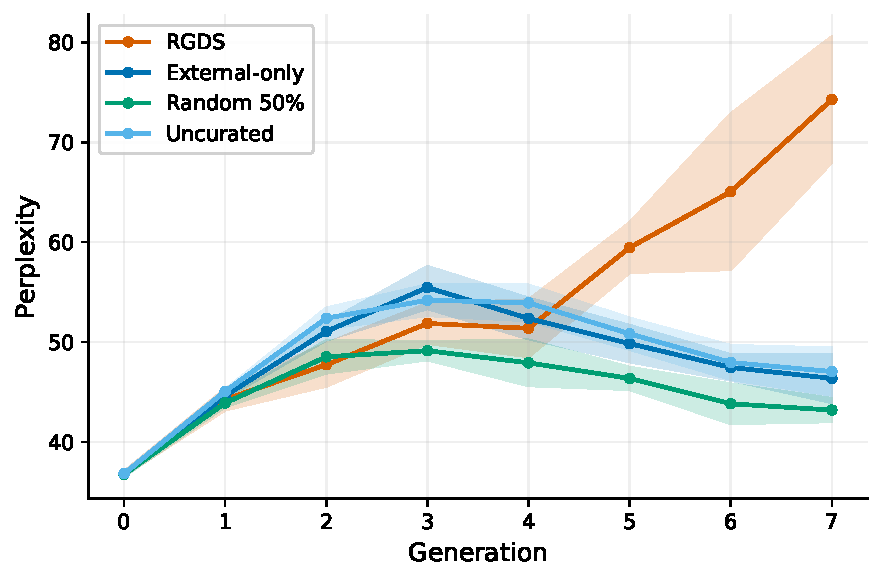
\includegraphics[width=\columnwidth]{figures/fig_ppl_trends.pdf}
\caption{Per-generation perplexity trajectories across four data selection methods (GPT2-125M on WikiText-103). Lines show means over $n{=}3$ seeds; shaded bands show $\pm$1 standard deviation. RGDS diverges from the non-RGDS cluster after Generation~4 and reaches catastrophic perplexity by Generation~7 ($74.29 \pm 7.71$), while the other three methods converge to a narrow band (43--47).}
\label{fig:ppl_trends}
\end{figure}

\begin{figure}[t]
\centering
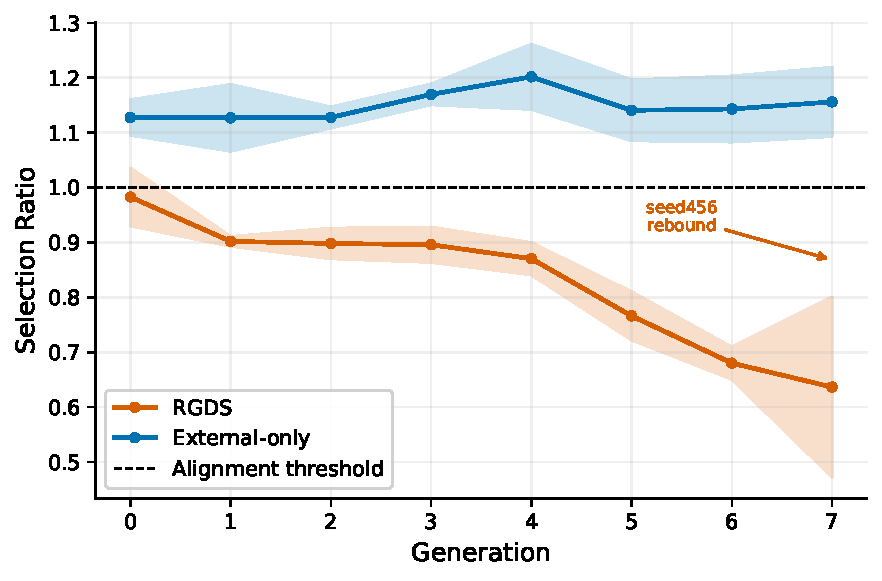
\includegraphics[width=\columnwidth]{figures/fig_ratio_trajectory.pdf}
\caption{Selection ratio trajectories for RGDS and External-only across eight generations. The dashed line marks the alignment threshold ($\text{SR}=1.0$): above it, the selected subset is richer in rare n-grams than the rejected subset; below it, the reverse. RGDS's mean ratio declines from ${\sim}1.0$ to $0.64 \pm 0.20$, while External-only remains above~1.0 throughout. The large variance at Generation~7 reflects seed=456's late rebound (0.65$\to$0.87) without perplexity recovery.}
\label{fig:ratio_trajectory}
\end{figure}

\subsection{RGDS Accelerates Catastrophic Perplexity Degradation}
\label{sec:result_c1}

RGDS is the only method that exhibits catastrophic performance degradation across generations. At Generation~7, RGDS reaches a perplexity of $74.29 \pm 7.71$ ($n{=}3$), compared to $47.04 \pm 2.90$ for Uncurated ($n{=}3$; +58\%) and $43.18 \pm 1.43$ for Random~50\% ($n{=}3$; +72\%). All three seeds show consistent catastrophic degradation---75.07 (seed=42), 81.57 (seed=123), and 66.22 (seed=456)---with all values far exceeding the 43--47 range of the non-RGDS methods. The inter-seed variance of RGDS ($\sigma = 7.71$) substantially exceeds that of any other method ($\sigma \leq 2.97$), reflecting the stochastic dynamics of the co-degradation feedback loop.

The selection ratio traces the mechanism behind this degradation (Figure~\ref{fig:ratio_trajectory}). RGDS's mean selection ratio follows an overall declining trend from ${\sim}1.0$ at Generation~0 to $0.64 \pm 0.20$ at Generation~7 ($n{=}3$). Seeds 42 and 123 reach deeply inverted ratios (0.52 and 0.52 respectively), while seed=456 exhibits a late-generation rebound from 0.65 at Generation~6 to 0.87 at Generation~7---without any corresponding improvement in perplexity (66.22 vs.\ 43--47 for non-RGDS methods). This dissociation between ratio recovery and perplexity indicates that once the embedding space has been sufficiently corrupted, even a partial restoration of selection alignment cannot reverse the accumulated damage to model quality. Across all seeds, the RGDS-selected subset contains fewer rare n-grams than the rejected subset.

\subsection{External Embeddings Avoid the Alignment Gap}
\label{sec:result_c2}

External-only selection applies the identical selection algorithm and 50\% data budget but uses frozen Contriever embeddings. It avoids catastrophic degradation entirely: its Generation~7 perplexity of $46.36 \pm 2.97$ ($n{=}3$) falls within the range of Uncurated ($47.04 \pm 2.90$) and Random~50\% ($43.18 \pm 1.43$).

External-only maintains a selection ratio above~1.0 throughout all generations ($1.16 \pm 0.08$ at Generation~7), indicating continued preferential retention of content-diverse samples.

Since RGDS and External-only differ in exactly one variable---the embedding source---the 27.9-point perplexity gap at Generation~7 ($74.29$ vs.\ $46.36$) is directly attributable to the use of co-degrading internal representations. The selection algorithm is not at fault; the failure is specific to coupling data selection to embeddings that co-evolve with the collapsing model.

Notably, External-only does not significantly outperform Random~50\% in perplexity ($46.36 \pm 2.97$ vs.\ $43.18 \pm 1.43$; $p = 0.198$, Welch's $t$-test, $n{=}3$). Despite maintaining a selection ratio above~1.0, the ``intelligent'' diversity signal from frozen external embeddings provides no measurable advantage over uninformed random subsampling. This null result reinforces the practical implication discussed in \S\ref{sec:discussion}: random sampling is a zero-cost alternative that matches the performance of embedding-guided selection when embeddings are stable and avoids the catastrophic failure when they are not.

\subsection{Internal Selection Underperforms Random Baseline}
\label{sec:result_c3}

The comparison between RGDS and Random~50\% constitutes the cleanest controlled ablation in our design. Both methods operate under identical conditions---same 50\% data budget, same training protocol, same seed infrastructure, same Generation~0 checkpoint---differing only in the selection mechanism: diversity-based curation via the model's own embeddings (RGDS) versus uninformed uniform sampling (Random~50\%). Any performance difference is therefore attributable solely to the selection mechanism, free from the data-volume confound present in comparisons against Uncurated (50\% vs.\ 100\%).

Under this controlled comparison, RGDS exhibits catastrophically worse performance. Its Generation~7 perplexity ($74.29 \pm 7.71$, $n{=}3$) exceeds Random~50\% ($43.18 \pm 1.43$, $n{=}3$) by $+$72\% ($p = .017$, Welch's $t$, $d = 5.61$). The effect is consistent across all three seeds, with each RGDS run (75.07, 81.57, 66.22) far exceeding the non-RGDS cluster ceiling of ${\sim}47$. Internal embedding diversity selection does not merely fail to improve upon random sampling---it actively degrades model quality by a margin that dwarfs all other method differences in this study.

Rare n-gram ratio corroborates the perplexity finding: RGDS retains $0.0061 \pm 0.0009$ at Generation~7, compared to $0.0098 \pm 0.0003$ for Random~50\%---a 38\% reduction in lexical tail content ($p = .014$, $d = -5.66$). The mechanism designed to maximize diversity produces outputs that are measurably \emph{less} diverse than those from uninformed subsampling.

This within-budget contrast should be distinguished from the RGDS vs.\ Uncurated comparison ($+$58\%), which conflates any selection effect with a data quantity difference (50\% vs.\ 100\%). The Random~50\% vs.\ Uncurated comparison (\S\ref{sec:result_s3}) similarly involves a budget confound and does not reach significance ($p = .133$), reinforcing that the within-budget RGDS-vs.-Random ablation provides the most interpretable causal evidence for the alignment gap.

\subsection{Random Pruning: A Directional Observation}
\label{sec:result_s3}

Random~50\% ($43.18 \pm 1.43$, $n{=}3$) achieves lower Generation~7 perplexity than Uncurated ($47.04 \pm 2.90$, $n{=}3$), a reduction of 8.2\% consistent across all three seeds. However, this cross-budget comparison conflates any selection benefit with a data quantity effect (50\% vs.\ 100\%), and the difference does not reach conventional significance ($p = 0.133$, Welch's $t$-test). We report it as a directional observation rather than a confirmed finding, and draw no causal inference about budget effects from this comparison alone.

If confirmed with additional statistical power, this result would suggest that training on a random 50\% subset provides mild regularization compared to using all generated data, consistent with observations that data pruning can improve generalization even without informed selection \citep{sorscher2022beyond}.

While the perplexity difference remains directional, Random~50\% shows a statistically significant advantage in lexical diversity: its Generation~7 rare n-gram ratio ($0.0098 \pm 0.0003$) exceeds Uncurated ($0.0090 \pm 0.0004$) with $p = 0.025$ (two-sided $t$-test, $n{=}3$). Even uninformed subsampling preserves content diversity better than retaining all generated data, suggesting that merely reducing the volume of self-generated training data slows lexical tail erosion.

\subsection{Lexical Diversity Collapse Across Methods}
\label{sec:result_diversity}

RGDS exhibits the sharpest decline in rare token ratio, dropping from approximately 0.010 at Generation~0 to $0.0061 \pm 0.0009$ at Generation~7 (Table~\ref{tab:gen7_summary}). The remaining methods converge to a narrower band: Random~50\% ($0.0098 \pm 0.0003$), Uncurated ($0.0090 \pm 0.0004$), and External-only ($0.0102 \pm 0.0004$). Relative to the WikiText-103 baseline rare token ratio of approximately 0.029, all non-RGDS methods exhibit roughly 65\% lexical tail erosion by Generation~7; RGDS reaches approximately 80\%.

Unlike the perplexity-level normal cluster (ANOVA $p = 0.219$; \S\ref{sec:result_c1}), the rare n-gram differences among non-RGDS methods are statistically significant (ANOVA $p = 0.007$, $n{=}3$ per method). In particular, Uncurated retains significantly fewer rare n-grams than Random~50\% ($p = 0.025$, two-sided $t$-test). Lexical diversity collapse is primarily driven by the iterative self-training loop itself \citep{shumailov2024ai}, but the degree of erosion is modulated by data selection: even uninformed curation (random subsampling) provides measurable protection relative to using all generated data. RGDS is distinctive in accelerating this inherent degradation far beyond all other methods.

\begin{table*}[t]
\centering
\small
\begin{tabular}{llrrrrl}
\toprule
Comparison & Metric & $\Delta$ & Welch $t$ & df & $p$ & Cohen's $d$ \\
\midrule
\multicolumn{7}{l}{\textit{RGDS vs.\ non-RGDS methods}} \\
RGDS vs.\ Random 50\% & PPL & $+$31.10 & 6.88 & 2.1 & .017 & 5.61 \\
RGDS vs.\ External-only & PPL & $+$27.93 & 5.86 & 2.6 & .015 & 4.78 \\
RGDS vs.\ Uncurated & PPL & $+$27.25 & 5.73 & 2.6 & .016 & 4.68 \\
RGDS vs.\ Random 50\% & Rare & $-$.0038 & $-$6.93 & 2.3 & .014 & $-$5.66 \\
RGDS vs.\ External-only & Rare & $-$.0042 & $-$7.51 & 2.6 & .008 & $-$6.13 \\
RGDS vs.\ Uncurated & Rare & $-$.0029 & $-$5.16 & 2.6 & .020 & $-$4.22 \\
\midrule
\multicolumn{7}{l}{\textit{Within-cluster comparisons}} \\
External vs.\ Random 50\% & PPL & $+$3.17 & 1.67 & 2.9 & .198 & 1.36 \\
Random 50\% vs.\ Uncurated & PPL & $-$3.86 & $-$2.07 & 2.9 & .133 & $-$1.69 \\
Random 50\% vs.\ Uncurated & Rare & $+$.0009 & 3.47 & 3.6 & .030 & 2.84 \\
\midrule
\multicolumn{7}{l}{\textit{ANOVA (one-way)}} \\
Non-RGDS (3 methods) & PPL & --- & $F{=}1.98$ & 2,\,6 & .219 & --- \\
Non-RGDS (3 methods) & Rare & --- & $F{=}13.01$ & 2,\,6 & .007 & --- \\
\midrule
\multicolumn{7}{l}{\textit{GPT2-Medium (355M)---$n{=}2$ seeds (42, 123); seed=456 pending}} \\
RGDS vs.\ Random 50\% & PPL & $+$15.15 & \multicolumn{3}{c}{---} & --- \\
RGDS vs.\ External-only & PPL & $+$7.90 & \multicolumn{3}{c}{---} & --- \\
RGDS vs.\ Uncurated & PPL & $-$2.81 & \multicolumn{3}{c}{---} & --- \\
Random 50\% vs.\ Uncurated & PPL & $-$17.96 & \multicolumn{3}{c}{---} & --- \\
\bottomrule
\end{tabular}
\caption{Pairwise statistical comparisons at Generation~7. GPT2-125M rows: $n{=}3$ seeds per method. All pairwise tests use Welch's $t$-test (two-sided, unequal variance). PPL: perplexity on WikiText-103 validation set. Rare: rare trigram ratio. $\Delta$: difference (row method $-$ column method for pairwise; not applicable for ANOVA). Cohen's $d$: standardized effect size. RGDS differs significantly from all non-RGDS methods on both metrics ($p < .05$, $|d| > 4$). Within the non-RGDS cluster, PPL differences are not significant (ANOVA $p = .219$), but rare n-gram differences are (ANOVA $p = .007$). 355M: $n{=}2$ seeds (42, 123); seed=456 pending; $t$-tests deferred until $n \geq 3$.}
\label{tab:stat_tests}
\end{table*}

\subsection{Representation Metrics Do Not Track Content Collapse}
\label{sec:result_rankme}

RankMe values at Generation~7 are comparable across all methods (289--293; Table~\ref{tab:gen7_summary}), with no method showing a meaningfully different value ($292.54 \pm 5.91$ for RGDS vs.\ ${\sim}290$ for non-RGDS methods). The metric designed to track effective embedding dimensionality does not distinguish between catastrophically degraded RGDS and the normally performing alternatives, indicating that embedding structural properties can persist even as the space loses content-discriminative fidelity.

\subsection{Scaling to GPT2-Medium (355M)}
\label{sec:result_scaling}

Results from GPT2-Medium (355M) confirm that model collapse generalizes to larger models and is substantially amplified. Table~\ref{tab:medium_comparison} reports Generation~7 perplexity for all four methods (seed=42 and seed=123 complete for all four methods; all seed=456 experiments pending).%
%TODO(355M-seeds): update when Random seed=123 and all seed=456 complete

\begin{table}[t]
\centering
\small
\begin{tabular}{lcccc}
\toprule
Method & Budget & PPL$_{42}$ & PPL$_{123}$ & $n$ \\
\midrule
Random 50\% & 50\% & 70.25 & 72.55 & 2 \\
External-only & 50\% & 77.74 & 79.56 & 2 \\
RGDS & 50\% & 82.84 & 90.25 & 2 \\
Uncurated & 100\% & 91.66 & 87.05 & 2 \\
\bottomrule
\end{tabular}
\caption{GPT2-Medium (355M) Generation~7 perplexity by seed. PPL$_{42}$ and PPL$_{123}$: WikiText-103 validation perplexity for each seed. RGDS and Uncurated ordering flips across seeds (82.84 vs.\ 91.66 at seed=42; 90.25 vs.\ 87.05 at seed=123). All seed=456 experiments are pending.}
\label{tab:medium_comparison}
\end{table}

\paragraph{C3 holds across scale.} The RGDS two-seed mean (86.55) underperforms Random~50\% (71.40) by +21\% at 355M ($n{=}2$), confirming that internal-embedding diversity selection degrades performance relative to uninformed random sampling regardless of model size. The gap is narrower than at 125M (+72\%, $n{=}3$), but the direction is consistent: co-degrading embeddings produce systematically worse selection than random chance.%
%TODO(355M-seeds): report significance with seed=456

\paragraph{Relative severity shifts at 355M.} At 355M, model collapse is substantially more severe than at 125M across all methods. RGDS and Uncurated converge into a narrow, overlapping band (PPL 83--92) with unstable ordering across seeds: RGDS outperforms Uncurated at seed=42 (82.84 vs.\ 91.66) but underperforms at seed=123 (90.25 vs.\ 87.05). This ordering instability contrasts sharply with the 125M setting, where RGDS consistently exceeded Uncurated by 58\% ($74.29$ vs.\ $47.04$, $n{=}3$). The compression of method differences at high absolute collapse severity is consistent with both the representational redundancy and floor-compression hypotheses discussed in \S\ref{sec:discuss_scaling}. The cross-budget comparison (50\% vs.\ 100\%) remains confounded by data volume differences and should not be interpreted causally. Only the within-budget comparison (RGDS vs.\ Random~50\%, both at 50\%) isolates the effect of the selection mechanism.%
%TODO(355M-seeds): update with seed=456 data

\paragraph{Alignment gap narrows but persists.} The RGDS selection ratio at Generation~7 is $0.85 \pm 0.03$ at 355M ($n{=}2$; 0.83 at seed=42, 0.87 at seed=123), compared to $0.64 \pm 0.20$ at 125M ($n{=}3$). The ratio remains below~1.0---RGDS still preferentially retains content-poor samples---but the inversion is less severe. The +21\% perplexity penalty relative to Random (vs.\ +72\% at 125M) is consistent with this narrower gap.%
%TODO(355M-seeds): confirm ratio trajectory with seed=123 完成后补充完整 4-method 对比和统计检验
